\chapter{Knowledge gain across episodes}
\begin{quotation}
\noindent ``\emph{Failure is simply the opportunity to begin again,
	this time more intelligently.}''
\begin{flushright}\textbf{Henry Ford}\end{flushright}
\end{quotation}
\vspace*{0.5cm}

\section{Meta-learning CartPole setting}
\label{sec:setting}
We will now go beyond the bandit experiments presented in Wang et al. 
\cite{learningtorl} and Duan et al. \cite{fastrlviaslowrl} and extend the study 
of the performance of meta-learning on multi-timestep
episodes; and for that purpose, we will use various distributions of 
the CartPole problem. The CartPole environment describes a cart, rolling on 
a frictionless rail (see Figure~\ref{fig:cartpole_illustration}). 
A pole is attached to the cart and has to be kept balanced
above the cart for more than 195 timesteps by also keeping the cart within a 
defined section of the rail. The agent has two actions at its disposal: nudge
the cart left or right. The observation of the state is a 4-valued vector 
containing the position of the cart, its velocity, the angle of the pole and
the velocity of the pole at its tip. At each time step, the environment emits
a reward of +1; so if the agent keeps the pole and the cart in their 
respective acceptable ranges for 20 timesteps, it will receive a total reward
of 20.\\


\subsection{Generating a distribution of CartPole problems}
To generate a distribution of similar, yet different CartPole problems, we
will play with two different parameters.

\paragraph{Permutations} In standard reinforcement learning, the state
observation vector is always ordered, meaning that each component of the vector
always represents the same value (in CartPole for example, the first component
represents the position of the cart). We can generate a set of $4! = 24$
CartPole problems where for each problem, the state observation vector is
permutated with a unique permutation. This means that the agent will
receive a vector of 4 values without knowing which is which.

\paragraph{Actions inversion} We will also introduce the inversion of the
agent's actions. Just like the input vector, the policy output is ordered
(the first component of the policy corresponds to the first action which is
always the same). We will study how inverting actions affects training : instead
of always associating the first component of the policy vector with going left,
we will duplicate each of the 24 problems stated above by inverting the left
and the right action. This adds up to a distribution of 48 CartPole problems.\\

Figure~\ref{fig:meta_cartpole} shows how the single-timestep framework
presented in Figure~\ref{fig:meta_bandit_training} adapts to episodes
with multiple timesteps.

\begin{figure}[H]
	\centering
	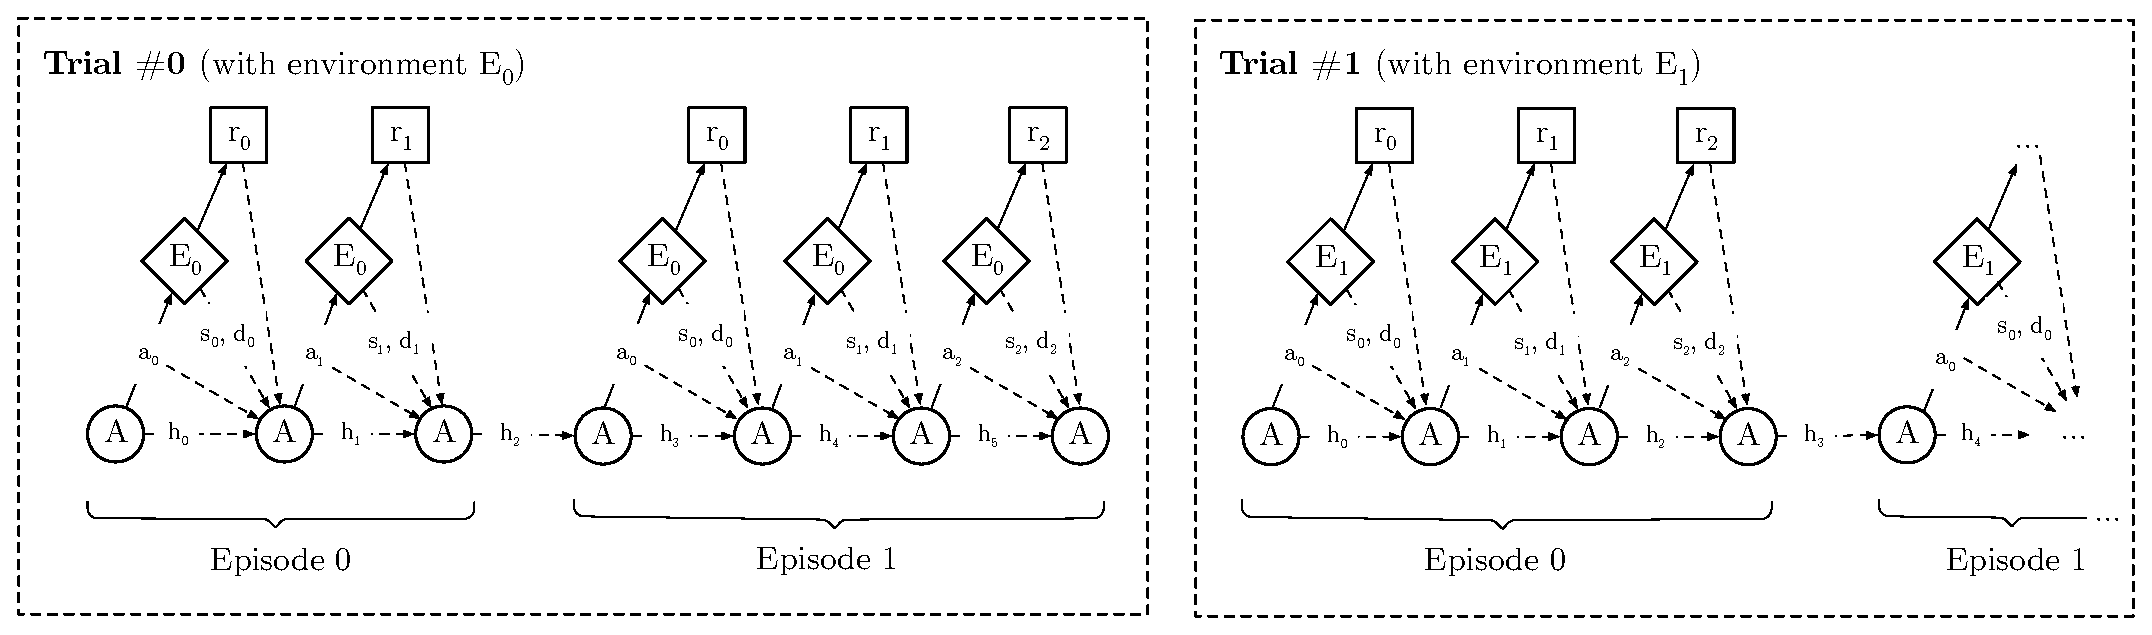
\includegraphics[width=\linewidth]{fig/meta_cartpole.eps}
	\caption{Meta-learning for multi-timestep episodes. A is the agent,
	$E_0$ is the problem selected from the distribution for the duration
	of a trial, $s_t$, is the state of the environment, $r_t$, the reward,
	$a_t$ is the chosen action, $d_t$ the terminal state and $h_t$ is
	the hidden state at timestep $t$. Note that the same environment is
	used throughout all episodes of the same trial.}
	\label{fig:meta_cartpole}
\end{figure}

\section{Performance gain when playing multiple episodes}

We will first and foremost analyse how a reinforcement learning agent 
performs when it is confronted to playing a single episode of one of the 
CartPole problems. We will train the agent on a distribution of 18 permutations
(shown in Table~\ref{tab:20perms}), at first without inverting the agent's
action.\\

\begin{table}
	\centering
	\caption{State permutations used for training and testing}
	\label{tab:20perms}
	\stackunder[5pt]{\small (a) Training distribution}{
		\bgroup
		\def\arraystretch{1.5}
		\begin{tabular}{c|c|c}
			[0, 1, 2, 3] & [1, 0, 2, 3] & [2, 0, 1, 3] \\
			\hline
			[0, 1, 3, 2] & [1, 0, 3, 2] & [2, 0, 3, 1] \\
			\hline
			[0, 2, 1, 3] & [1, 2, 0, 3] & [2, 1, 0, 3] \\
			\hline
			[0, 2, 3, 1] & [1, 2, 3, 0] & [3, 0, 1, 2] \\
			\hline
			[0, 3, 1, 2] & [1, 3, 0, 2] & [3, 0, 2, 1] \\
			\hline
			[0, 3, 2, 1] & [1, 3, 2, 0] & [3, 1, 0, 2] 
		\end{tabular}
		\egroup
	}
	\stackunder[5pt]{\small (b) Testing distribution}{
		\quad\quad
		\bgroup
		\def\arraystretch{1.5}
		\begin{tabular}{c}
			[2, 1, 3, 0] \\
			\hline
			[2, 3, 0, 1] \\
			\hline
			[2, 3, 1, 0] \\
			\hline
			[3, 1, 2, 0] \\
			\hline
			[3, 2, 0, 1] \\
			\hline
			[3, 2, 1, 0]
		\end{tabular}
		\egroup
		\quad\quad
	}
\end{table}

As a control experiment, we first need to check whether the agent can learn
to discover which permutation of the state has been selected and to keep the
pole balanced within one single episode. Surprisingly, as shown in 
Figure~\ref{fig:20perms1ep_training}, the agent quickly manages to reach
a very good performance level, only failing a small percentage of the time.\\

\begin{figure}[H]
	\centering
	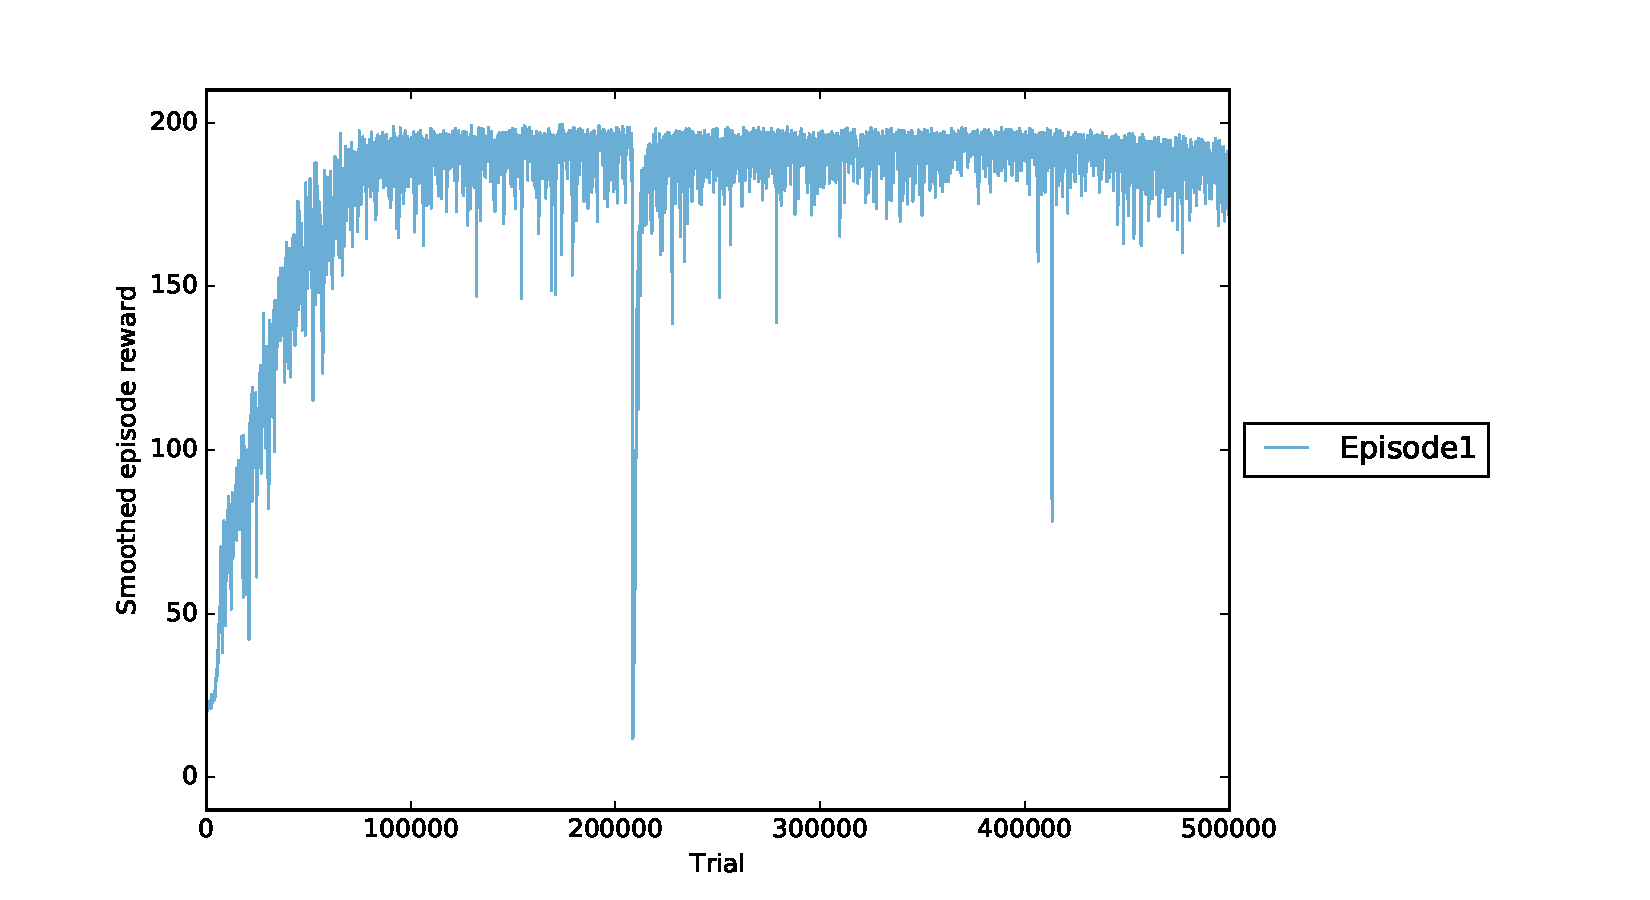
\includegraphics[width=0.9\linewidth]{fig/20perms1ep_training.pdf}
	\caption{Training of an agent on trials of 1 episode. The curve
	shows a moving average over 200 trials.}
	\label{fig:20perms1ep_training}
\end{figure}

When the agent is trained on trials of 2 episodes, we expect that its
performance will improve (however good it already is). Looking at the graph 
of Figure~\ref{fig:20perms2ep_training}, we can only deduce two things : 
\begin{enumerate}
	\item the performance of the first episode of every trial drops 
		significantly compared to trials of one episode;
	\item the performance of the second episode of every trial matches
		closely the performance of single-episode trials.
\end{enumerate}

\begin{figure}[H]
	\centering
	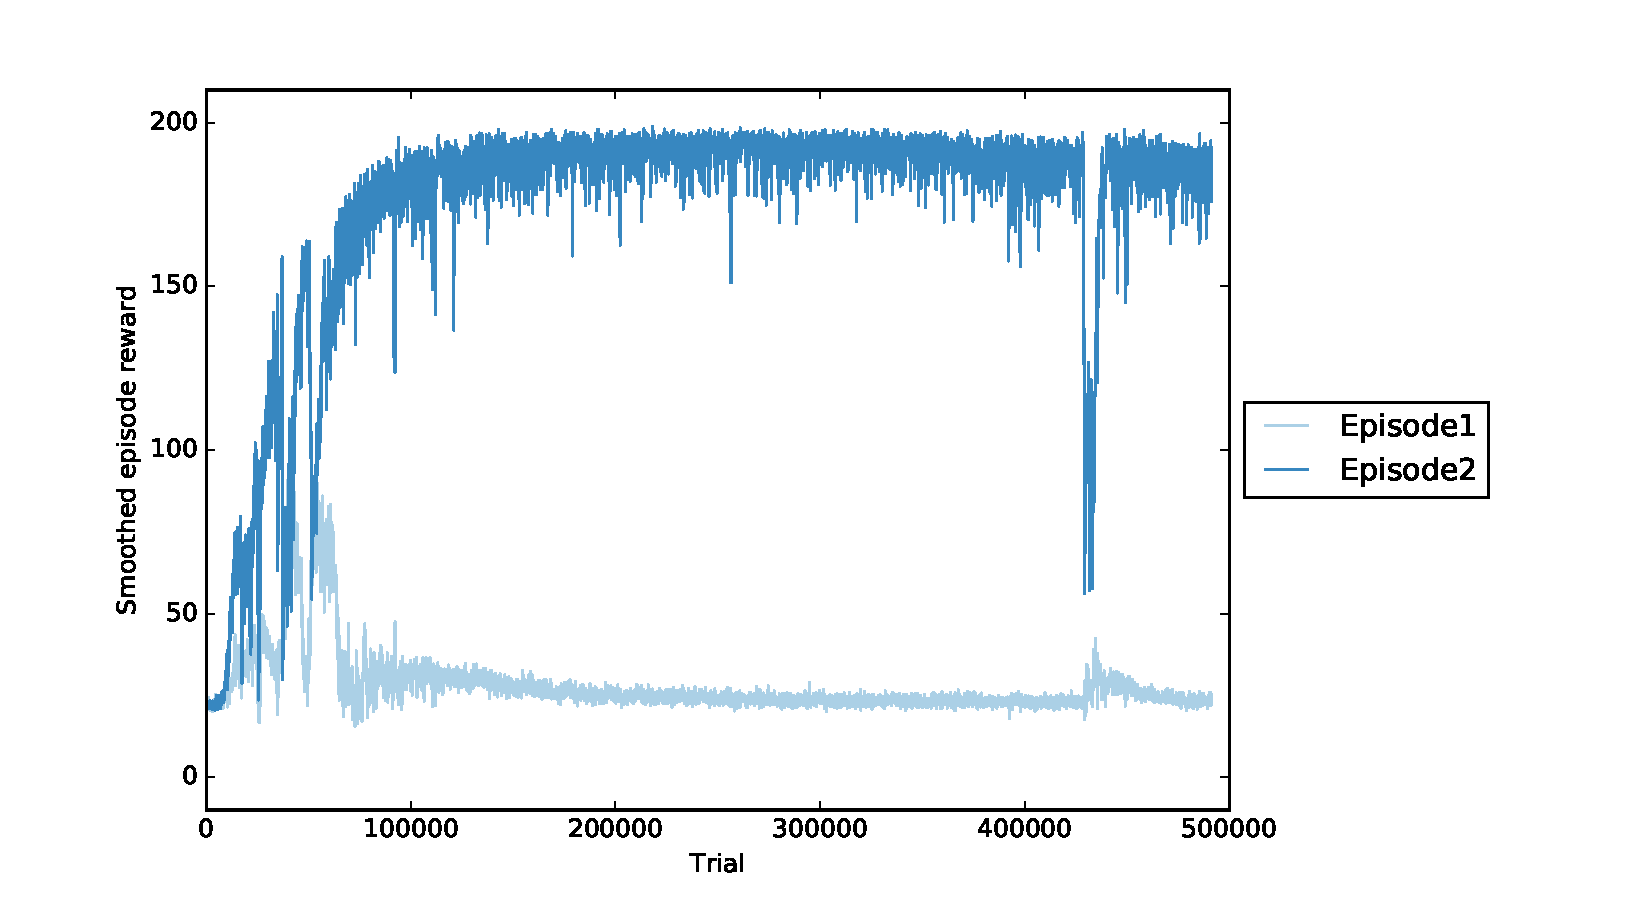
\includegraphics[width=0.9\linewidth]{fig/20perms2ep_training.pdf}
	\caption{Training of an agent on trials of 2 episodes}
	\label{fig:20perms2ep_training}
\end{figure}

The first of these considerations will be addressed in
chapter~\ref{chap:reward_structure}. Let us analyse the second one in more detail
as the average reward graph doesn't give us enough insight in the final
reward distributions.\\


Let us compare the final reward distribution for the only episode of 
single-episode trials and for the second episode of dual-episode trials.
For now, we are not interested in the reward distribution of the first episode
in dual-episode trials as we want to see whether or not the agent managed to
gain knowledge during that first episode (potentially hurting its first episode
reward) to improve its performance for the second episode.\\

\begin{figure}[H]
	\centering
	\subfloat[][Trials of 1 episode]{
		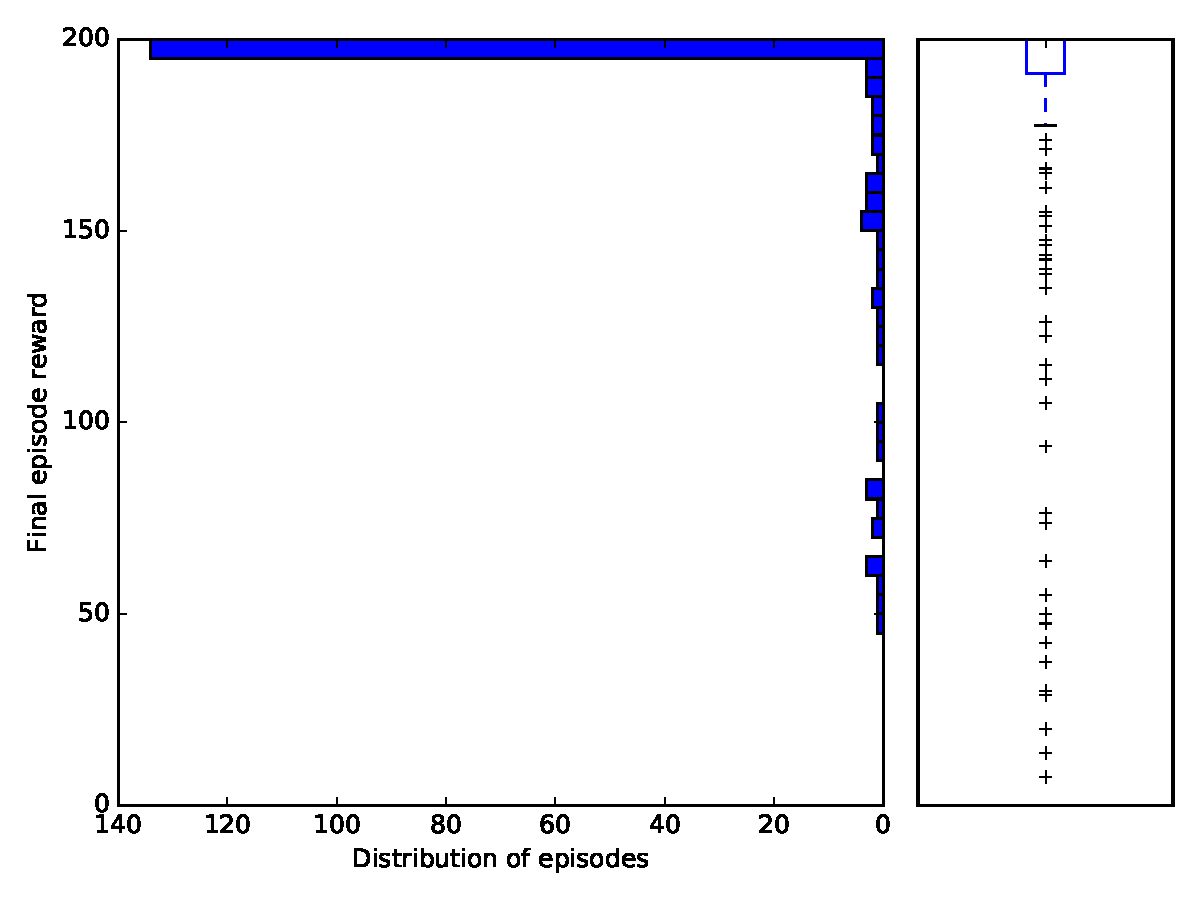
\includegraphics[width=0.49\linewidth]{fig/20perms_distrib_1ep.pdf}}
	\subfloat[][Trials of 2 episodes]{
		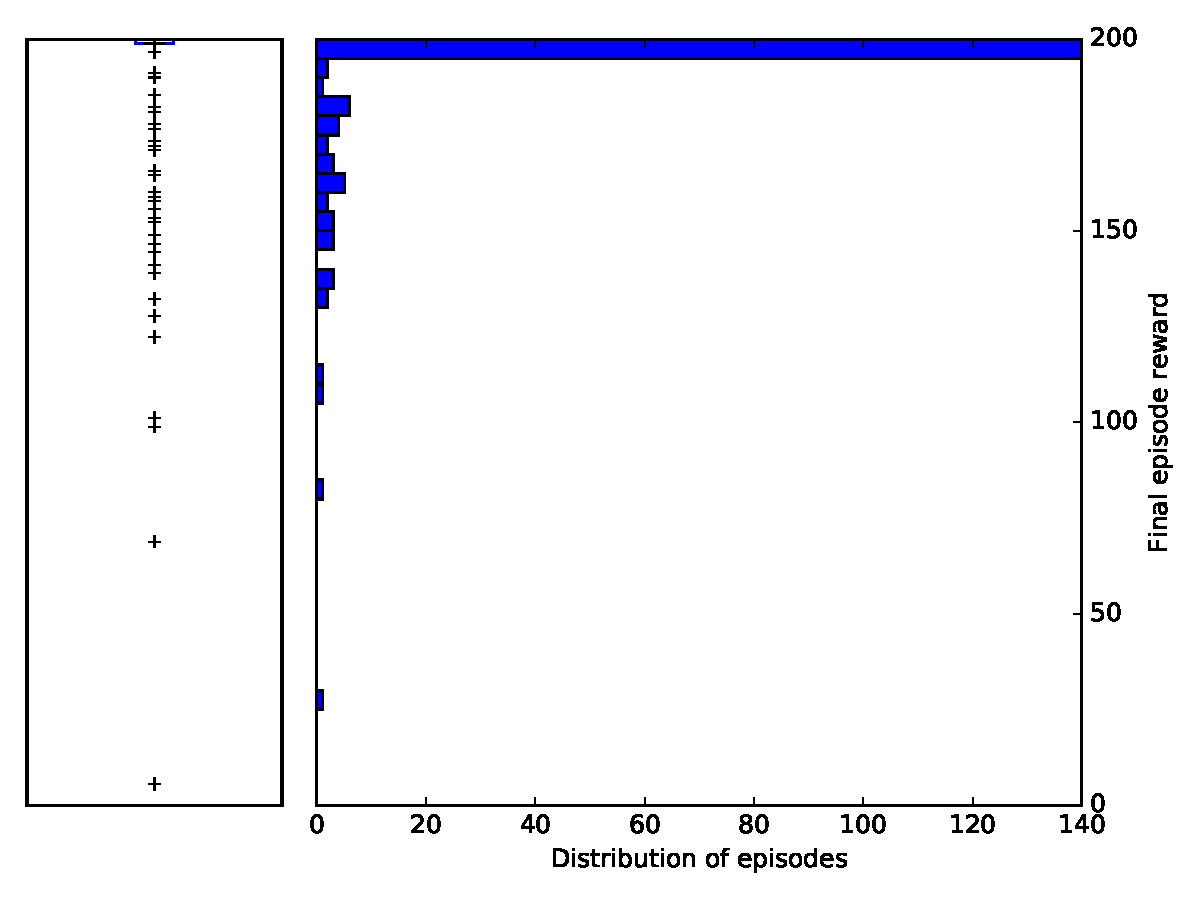
\includegraphics[width=0.49\linewidth]{fig/20perms_distrib_2ep.pdf}}
	\caption{Distributions of the total reward accumulated during the last
	episode of trials. 180 trials are played both in the case of
	single-episode trials and dual-episode trials. This shows the
	distribution of rewards obtained after playing 10 times each
	permutation of the \textbf{training} set. No action inversion is performed.}
	\label{fig:20perms_distrib}
\end{figure}

\begin{figure}[H]
	\centering
	\subfloat[][Trials of 1 episode]{
		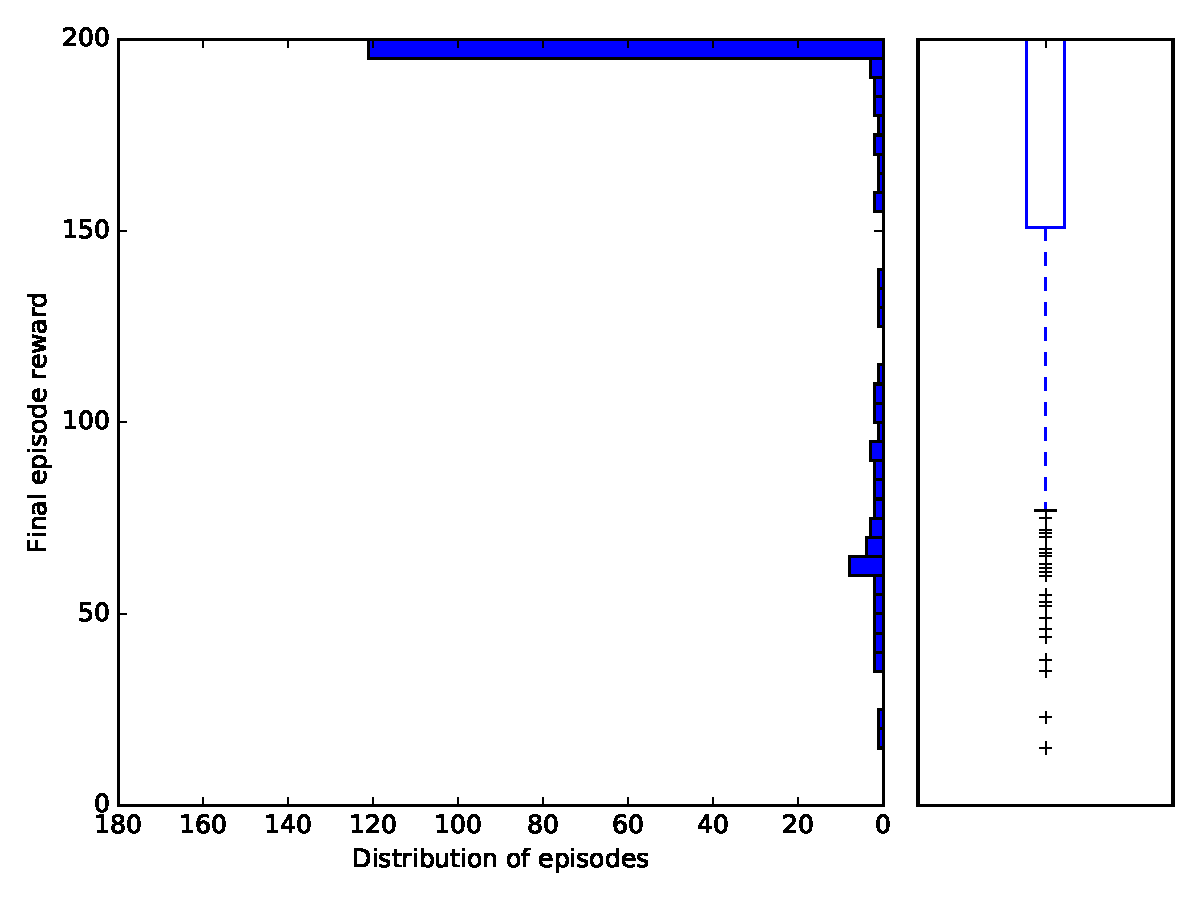
\includegraphics[width=0.49\linewidth]{fig/20perms_unseen_distrib_1ep.pdf}}
	\subfloat[][Trials of 2 episodes]{
		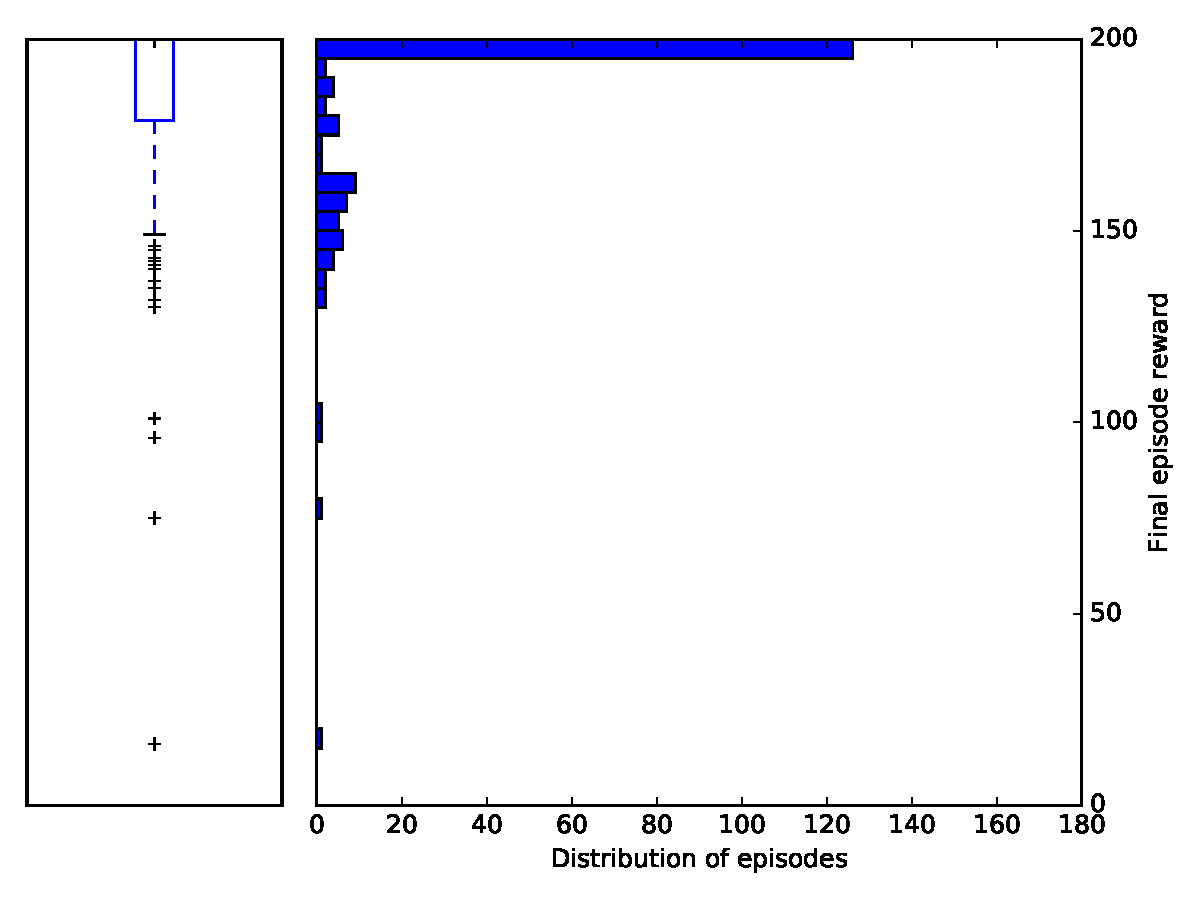
\includegraphics[width=0.49\linewidth]{fig/20perms_unseen_distrib_2ep.pdf}}
	\caption{Distributions of the total reward accumulated during the last
	episode of trials. This shows the distribution of rewards obtained
	after playing 30 times each permutation of the \textbf{test} set. No action
	inversion is performed.}
	\label{fig:20perms_unseen_distrib}
\end{figure}

To compare the two settings, we fix the agent's learnable parameters and make
it play 180 trials (resetting its hidden state before every trial). Every 
CartPole problem in the distribution is played the same amount of times.
Fixing the agent's learnable parameters means that we do not change
any of the weights of the neural network that represents the meta-learning
agent. We should perhaps emphasize that this means we do not train the agent
anymore; and that we expect the agent to learn \textbf{after training} still,
even though its weights are fixed.\\

Figure~\ref{fig:20perms_distrib} shows both a histogram and a boxplot describing
the final reward distributions in the single and dual episode situations. 
Although the difference is slight, and seeing that the number
of successes (a final reward of 195 or more, corresponding to the uppermost
bar) is almost exactly the same, there is definitely a difference in when the
failures occur. For the single episode setting, all failures are distributed
in a relatively uniform way spanning from 50 to 195; whereas they cluster 
slightly above 150 in the dual episode setting. The boxplots clearly show
a more compact distribution (and so a generally higher reward) in the dual
episode setting.\\

The agent seems to learn from the first episode to improve its performance in
the second. This is even clearer when we run the same experiment on unseen
permutations. As shown on Figure~\ref{fig:20perms_unseen_distrib}, where the
agent played every permutation of the test set for 30 trials, playing 180
trials in total to allow for comparison to the previous experiment, the agent
playing single-episode trials fails more often with a reward around 50. The
dual-episode setting shows again a capability to learn from the first episode
to improve performance in the second. We will later analyse performance
with longer trials containing more episodes.\\

Even more impressingly, if we add the inversion of the left and right actions
with a probability of 0.5 at the start of every trial, this effect is
tremendously magnified. For seen permutations
(Figure~\ref{fig:20permsLR_distrib}), there are about 40 more successes (out of
180) when playing two episodes than when playing only one; for unseen
permutations, this number climbs to about 70 out of 180. The single-episode
agent succeeds shy of 100 trials out of 180 where the dual-episode agent
comes close to 170 out of 180.\\

The reader might have noticed that the absolute performance for the agent
playing dual-episode trials is better when the problem is harder (with
inverted actions) as it succeeds close to 170 trials out of 180 whereas
for the simpler problem (without inverted actions), it only succeeds for
around 120 trials out of 180. We can only speculate as to why this result
occurs. We suggest this might be due to the fact that the harder problem
is impossible to be learned in one epiosde, thus forcing the agent to
really become a meta-learning agent, making it perform extremely well during
the second episode; whereas the simple problem might only be learned like
a standard reinforcement learning problem.\\

\begin{figure}
	\centering
	\subfloat[][Trials of 1 episode]{
		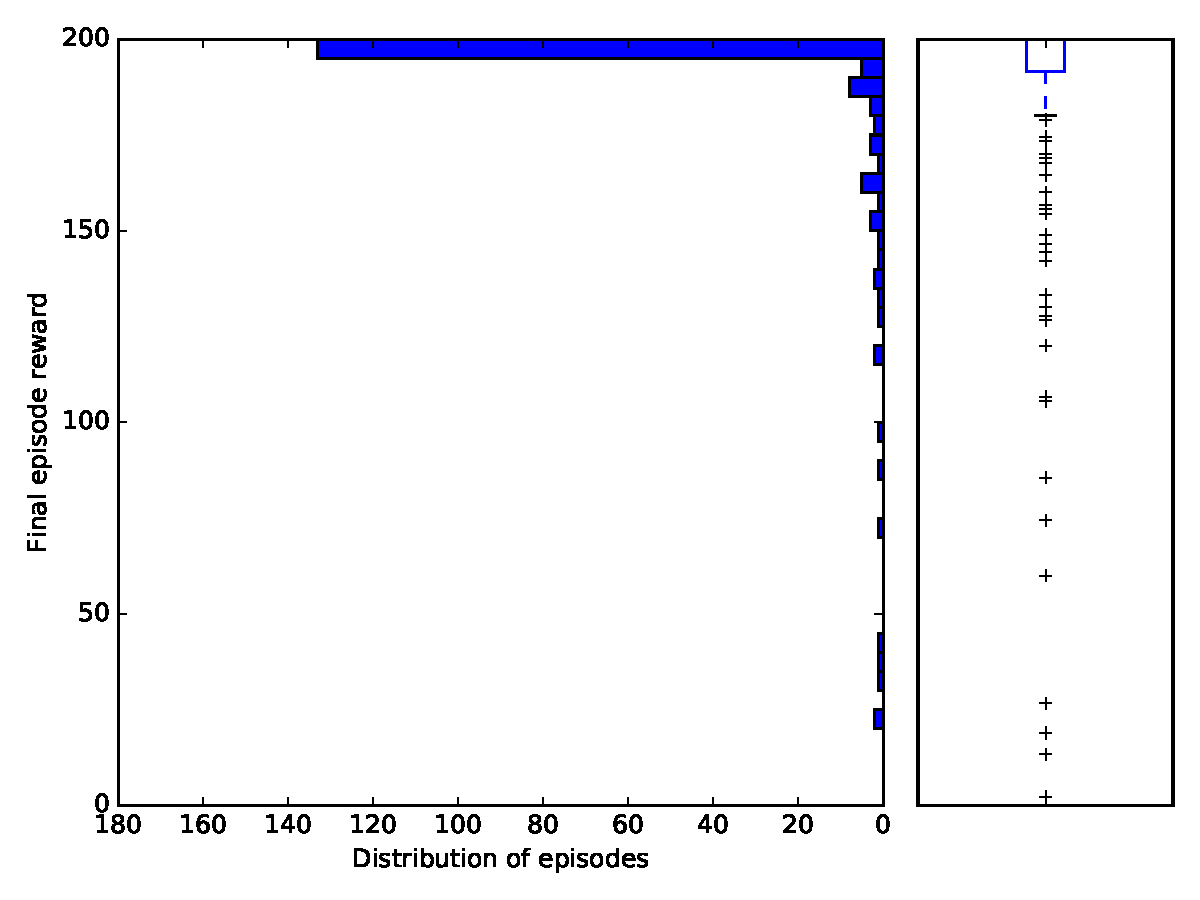
\includegraphics[width=0.49\linewidth]{fig/20permsLR_distrib_1ep.pdf}}
	\subfloat[][Trials of 2 episodes]{
		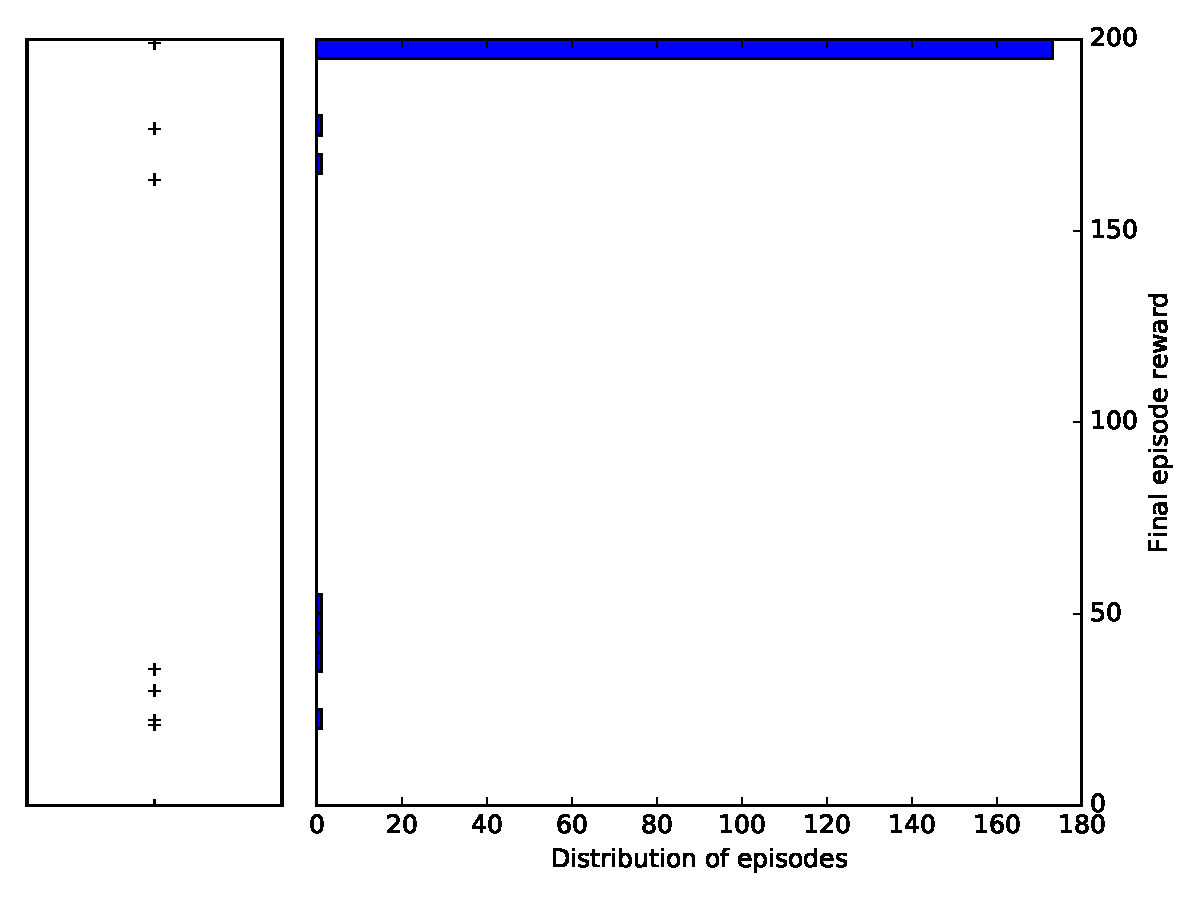
\includegraphics[width=0.49\linewidth]{fig/20permsLR_distrib_2ep.pdf}}
	\caption{Distributions of the total reward accumulated during the last
	episode of trials. This shows the distribution of rewards obtained after
	playing each permutation of the \textbf{training} set 5 times with action 
	inversion and 5 times without action inversion.}
	\label{fig:20permsLR_distrib}
\end{figure}

\begin{figure}
	\centering
	\subfloat[][Trials of 1 episode]{
		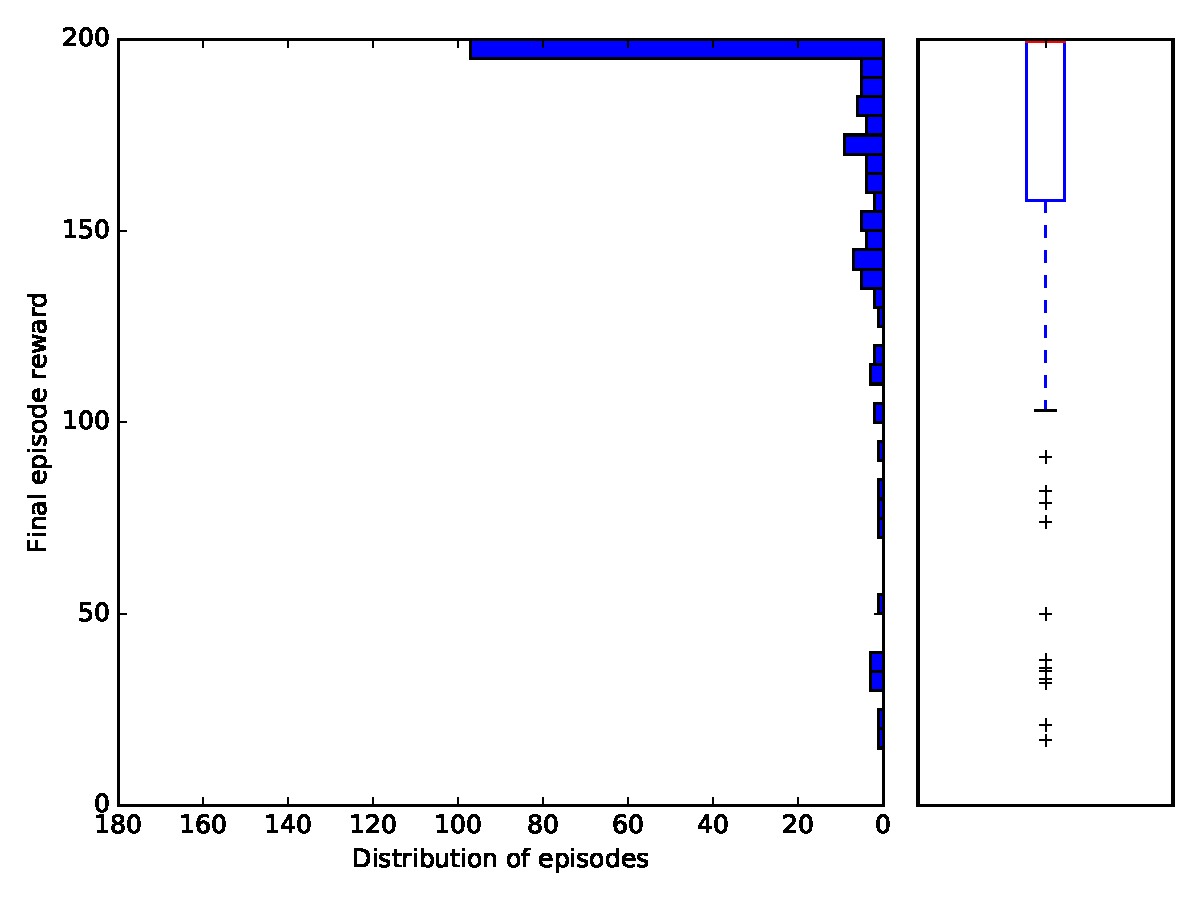
\includegraphics[width=0.49\linewidth]{fig/20permsLR_unseen_distrib_1ep.pdf}}
	\subfloat[][Trials of 2 episodes]{
		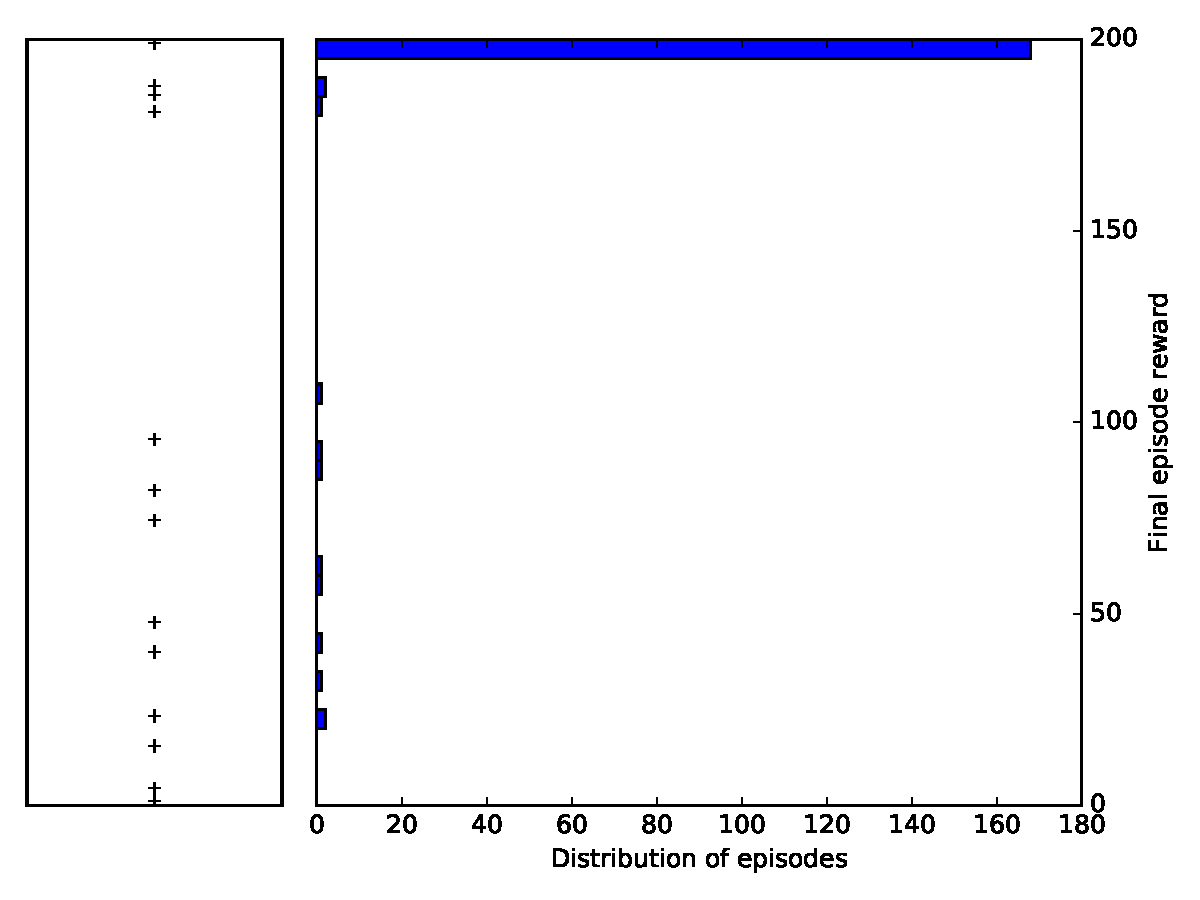
\includegraphics[width=0.49\linewidth]{fig/20permsLR_unseen_distrib_2ep.pdf}}
	\caption{Distributions of the total reward accumulated during the last
	episode of trials. This shows the distribution of rewards obtained after
	playing each permutation of the \textbf{test} set 5 times with action 
	inversion and 5 times without action inversion.}
	\label{fig:20permsLR_unseen_distrib}
\end{figure}

There are several surprises in these results. The first one is that a single
episode appears to be enough for an agent to discover how the observation has
been permutated in time to take action so that the pole stays balanced (at least
for a majority of trials), but playing a second episode improves the performance
of the agent (although at the cost of the reward of the first episode -- this
will be analysed in chapter~\ref{chap:reward_structure}).\\

The second one seems to be that in the setting of dual-episode trials, the
harder the problem is, the higher the number of successes will be. Indeed,
the performance of agents playing problems with inverted actions is 
significantly higher than the performance of agents playing problems without.


\subsubsection{Conclusion}
We have seen that applying meta-learning to a problem such as CartPole yields
interesting results on several aspects. The first one is that we can
indeed see information being passed from episode to episode to improve 
performance (in essence, learning is happening), but at the same some
behaviours deserve looking into:
\begin{itemize}
	\item the reward per episode seems to change quite a lot as a function
		of the number of episodes per trial and shows curious
		dynamics
	\item harder problems seem to make meta-learning more effective than
		simple problems; not only is the difference between 
		non-meta-learning and meta learning larger, but the absolute
		performance of the meta-learning agent on a harder problem
		is better than the absolute performance of the meta-learning
		agent on a simpler problem.
\end{itemize}

We will now look into more details as to why these behaviours occur.





